% ============================================================
\chapter{Persistent Homology}
\label{ch:persistent}
% ============================================================

Classical homology answers the question: ``how many holes does this space have?'' But in topological data analysis, the space itself is not given---we only have a point cloud, and the topology depends on the scale parameter chosen. At a small scale, every point is isolated; at a large scale, everything merges into a single connected component. The question becomes: ``which topological features \emph{persist} across scales?'' This is the founding idea of persistent homology, developed in the early 2000s by Herbert Edelsbrunner, David Letscher, and Afra Zomorodian, then enriched by Gunnar Carlsson and his collaborators.

The key result is that persistence can be represented by a \emph{persistence diagram}: a set of points in the plane, where each point $(b, d)$ encodes the birth and death of a topological feature. Points far from the diagonal correspond to robust structures; those near the diagonal are noise. This representation, both simple and powerful, has become the central tool of TDA.

\begin{intuition}
Classical homology describes the topology of a fixed space. \emph{Persistent}
homology studies how this topology \emph{evolves} as one traverses a nested
family of complexes: it detects when a topological feature is born and
when it dies.
\end{intuition}

% ============================================================
\section{Filtrations}
% ============================================================

\begin{definition}[Filtration of a Simplicial Complex]
A \emph{filtration} of a simplicial complex $K$ is an increasing
sequence of subcomplexes:
\[
  \emptyset = K_0 \subseteq K_1 \subseteq K_2 \subseteq \cdots
  \subseteq K_m = K
\]
where each $K_i$ is a subcomplex of $K$.
\end{definition}

\begin{definition}[Function-Induced Filtration]
Equivalently, a filtration can be described by a function
$f : K \to \R$ such that for every $\sigma \in K$ and every face
$\tau \subseteq \sigma$, $f(\tau) \leq f(\sigma)$. The filtered
complex at level $r$ is:
\[
  K_r = f^{-1}((-\infty, r]) = \{\sigma \in K : f(\sigma) \leq r\}.
\]
\end{definition}

\begin{example}[Vietoris--Rips Filtration]
Given a point cloud $X \subset \R^d$, the Vietoris--Rips filtration is:
\[
  \mathrm{VR}(X, r) = \big\{
    \sigma \subseteq X : \norm{x_i - x_j} \leq 2r
    \;\text{for all}\; x_i, x_j \in \sigma
  \big\}.
\]
As $r$ increases, more and more simplices appear.
\end{example}

\begin{center}
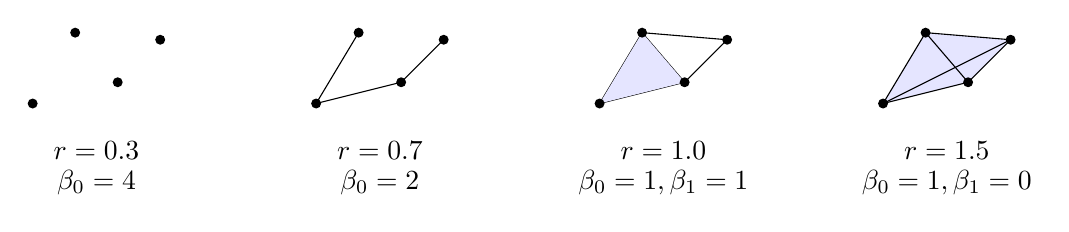
\begin{tikzpicture}[scale=0.9]
  % r = 0.3
  \begin{scope}[shift={(0,0)}]
    \foreach \p in {(0,0),(1.2,0.3),(0.6,1.0),(1.8,0.9)}{
      \fill \p circle (2pt);
    }
    \node[below] at (0.9,-0.4) {$r = 0.3$};
    \node[below] at (0.9,-0.8) {$\beta_0 = 4$};
  \end{scope}
  % r = 0.7
  \begin{scope}[shift={(4,0)}]
    \draw (0,0) -- (1.2,0.3);
    \draw (0,0) -- (0.6,1.0);
    \draw (1.2,0.3) -- (1.8,0.9);
    \foreach \p in {(0,0),(1.2,0.3),(0.6,1.0),(1.8,0.9)}{
      \fill \p circle (2pt);
    }
    \node[below] at (0.9,-0.4) {$r = 0.7$};
    \node[below] at (0.9,-0.8) {$\beta_0 = 2$};
  \end{scope}
  % r = 1.0
  \begin{scope}[shift={(8,0)}]
    \draw (0,0) -- (1.2,0.3) -- (0.6,1.0) -- cycle;
    \draw (1.2,0.3) -- (1.8,0.9) -- (0.6,1.0);
    \fill[blue!10] (0,0) -- (1.2,0.3) -- (0.6,1.0) -- cycle;
    \foreach \p in {(0,0),(1.2,0.3),(0.6,1.0),(1.8,0.9)}{
      \fill \p circle (2pt);
    }
    \node[below] at (0.9,-0.4) {$r = 1.0$};
    \node[below] at (0.9,-0.8) {$\beta_0 = 1, \beta_1 = 1$};
  \end{scope}
  % r = 1.5
  \begin{scope}[shift={(12,0)}]
    \fill[blue!10] (0,0) -- (1.2,0.3) -- (0.6,1.0) -- cycle;
    \fill[blue!10] (1.2,0.3) -- (1.8,0.9) -- (0.6,1.0) -- cycle;
    \draw (0,0) -- (1.2,0.3) -- (1.8,0.9) -- (0.6,1.0) -- cycle;
    \draw (1.2,0.3) -- (0.6,1.0);
    \draw (0,0) -- (1.8,0.9);
    \foreach \p in {(0,0),(1.2,0.3),(0.6,1.0),(1.8,0.9)}{
      \fill \p circle (2pt);
    }
    \node[below] at (0.9,-0.4) {$r = 1.5$};
    \node[below] at (0.9,-0.8) {$\beta_0 = 1, \beta_1 = 0$};
  \end{scope}
\end{tikzpicture}
\end{center}

% ============================================================
\section{Persistent Homology: Definition}
% ============================================================

\begin{definition}[Persistent Homology Groups]
Given a filtration $K_0 \subseteq K_1 \subseteq \cdots \subseteq K_m$,
the inclusion $\iota_{i,j} : K_i \hookrightarrow K_j$ ($i \leq j$)
induces a linear map in homology:
\[
  \iota_{i,j}^p : H_p(K_i) \to H_p(K_j).
\]
The \emph{$p$-th persistent homology group} from $K_i$ to $K_j$ is:
\[
  H_p^{i,j} = \mathrm{im}(\iota_{i,j}^p).
\]
The \emph{persistent Betti number} is
$\beta_p^{i,j} = \dim H_p^{i,j}$.
\end{definition}

\begin{definition}[Birth and Death]
A homology class $\gamma \in H_p(K_i)$ is \emph{born} at time $i$ if
$\gamma \notin \mathrm{im}(\iota_{i-1,i}^p)$. It \emph{dies} at time
$j > i$ if $\iota_{i,j-1}^p(\gamma) \neq 0$ but
$\iota_{i,j}^p(\gamma) = 0$. Its \emph{persistence} is $j - i$.
\end{definition}

\begin{keyformulas}[title=\textbf{Persistent Betti Numbers}]
\[
  \beta_p^{i,j} = \dim \frac{Z_p(K_i)}{B_p(K_j) \cap Z_p(K_i)}
\]
\end{keyformulas}

% ============================================================
\section{The Decomposition Theorem}
% ============================================================

\begin{definition}[Persistence Module]
A \emph{persistence module} (over $\mathbb{F}$) is a diagram of the
form:
\[
  V_1 \xrightarrow{\varphi_1} V_2 \xrightarrow{\varphi_2}
  \cdots \xrightarrow{\varphi_{m-1}} V_m
\]
where the $V_i$ are finite-dimensional vector spaces and the
$\varphi_i$ are linear maps.
\end{definition}

\begin{theorem}[Decomposition --- Crawley-Boevey, Gabriel]
Every \emph{pointwise finite-dimensional} persistence module over
$(\R, \leq)$ decomposes uniquely (up to isomorphism and permutation)
as a direct sum of interval modules:
\[
  \mathbf{V} \cong \bigoplus_{k=1}^{N} \mathbb{I}[b_k, d_k)
\]
where $\mathbb{I}[b, d)$ equals $\mathbb{F}$ on $[b, d)$ and $0$
elsewhere. The collection of pairs $\{(b_k, d_k)\}$ is the
\emph{persistence diagram}.
\end{theorem}

\begin{remark}
This theorem is the persistence-module analogue of the structure theorem
for modules over a PID (classification of graded modules over
$\mathbb{F}[t]$ due to Zomorodian--Carlsson, 2005).
\end{remark}

% ============================================================
\section{The Standard Algorithm}
% ============================================================

The boundary matrix reduction algorithm is the classical method for
computing persistent homology.

\begin{definition}[Filtered Boundary Matrix]
Order the simplices $\sigma_1, \ldots, \sigma_N$ of $K$ so that
$f(\sigma_i) \leq f(\sigma_j)$ for $i < j$ (where $f$ is the
filtration function), and faces appear before the simplices containing
them. The \emph{filtered boundary matrix} $D$ is the $N \times N$
matrix whose entry $(i, j)$ is the coefficient of $\sigma_i$ in
$\partial \sigma_j$.
\end{definition}

\begin{algorithme}[title=\textbf{Boundary Matrix Reduction}]
\begin{enumerate}
  \item Let $D$ be the filtered boundary matrix ($N \times N$).
  \item Define $\mathrm{low}(j)$ as the index of the lowest non-zero
        row in column $j$ (or $-1$ if the column is zero).
  \item For $j = 1, \ldots, N$:
    \begin{enumerate}
      \item While there exists $j' < j$ with
            $\mathrm{low}(j') = \mathrm{low}(j) \neq -1$:
      \item Add column $j'$ to column $j$ (over $\mathbb{F}$).
    \end{enumerate}
  \item After reduction:
    \begin{itemize}
      \item If $\mathrm{low}(j) = i$, then $(\sigma_i, \sigma_j)$
            forms a birth-death pair.
      \item If column $j$ is zero and $j$ is not the image of any
            $\mathrm{low}$, then $\sigma_j$ is an essential generator
            (never dies).
    \end{itemize}
\end{enumerate}
\end{algorithme}

\begin{codeblock}[title=\textbf{Matrix Reduction in Python}]
\begin{minted}{python}
def reduce_boundary_matrix(D):
    """Standard boundary matrix reduction over F_2.
    D: list of sets, D[j] = set of nonzero row indices of col j.
    Returns: pairs (birth, death) and essential generators.
    """
    n = len(D)
    pivot_col = {}  # maps pivot row -> column index
    pairs = []

    for j in range(n):
        while D[j] and max(D[j]) in pivot_col:
            j_prime = pivot_col[max(D[j])]
            D[j] = D[j].symmetric_difference(D[j_prime])

        if D[j]:
            i = max(D[j])
            pivot_col[i] = j
            pairs.append((i, j))

    return pairs

# Example: hollow triangle [a, b, c] with edges
# Order: a(0), b(1), c(2), ab(3), bc(4), ac(5)
D = [set(), set(), set(),
     {0, 1}, {1, 2}, {0, 2}]
pairs = reduce_boundary_matrix(D)
print("Pairs (birth, death):", pairs)
\end{minted}
\end{codeblock}

% ============================================================
\section{Algorithmic Complexity}
% ============================================================

\begin{theorem}[Complexity of the Standard Algorithm]
The boundary matrix reduction algorithm has worst-case complexity
$O(N^3)$, where $N$ is the total number of simplices in the filtration.
\end{theorem}

\begin{remark}
In practice, the matrix is very sparse and the algorithm runs much
faster. Optimizations like the \emph{clearing optimization} and the
\emph{twist} considerably reduce computation time. The \texttt{ripser}
implementation exploits these optimizations along with implicit matrix
reduction.
\end{remark}

% ============================================================
\section{Persistent Homology with Ripser}
% ============================================================

\begin{codeblock}[title=\textbf{Computation with Ripser}]
\begin{minted}{python}
import numpy as np
from ripser import ripser

# Generate points on a noisy circle
n = 100
theta = np.linspace(0, 2*np.pi, n, endpoint=False)
X = np.column_stack([np.cos(theta), np.sin(theta)])
X += 0.05 * np.random.randn(n, 2)

# Persistent homology up to dimension 1
result = ripser(X, maxdim=1)
dgm0 = result['dgms'][0]  # H_0
dgm1 = result['dgms'][1]  # H_1

print(f"H_0: {len(dgm0)} pairs")
print(f"H_1: {len(dgm1)} pairs")

# Most persistent pair in H_1
if len(dgm1) > 0:
    pers = dgm1[:, 1] - dgm1[:, 0]
    idx = np.argmax(pers)
    print(f"Most persistent H_1 pair: "
          f"birth={dgm1[idx,0]:.3f}, "
          f"death={dgm1[idx,1]:.3f}, "
          f"persistence={pers[idx]:.3f}")
\end{minted}
\end{codeblock}

% ============================================================
\section{Persistent Homology with GUDHI}
% ============================================================

\begin{codeblock}[title=\textbf{Computation with GUDHI}]
\begin{minted}{python}
import gudhi
import numpy as np

# Data: noisy circle
n = 100
theta = np.linspace(0, 2*np.pi, n, endpoint=False)
X = np.column_stack([np.cos(theta), np.sin(theta)])
X += 0.05 * np.random.randn(n, 2)

# Rips complex
rips = gudhi.RipsComplex(points=X, max_edge_length=2.0)
st = rips.create_simplex_tree(max_dimension=2)

# Persistence
persistence = st.persistence()
betti = st.betti_numbers()

print(f"Betti numbers: {betti}")
gudhi.plot_persistence_diagram(persistence)
\end{minted}
\end{codeblock}

% ============================================================
\section{Persistence Modules and Quiver Representations}
% ============================================================

\begin{definition}[Quiver $A_n$]
The quiver $A_n$ is the directed graph:
\[
  1 \to 2 \to 3 \to \cdots \to n.
\]
A (discrete, length-$n$) persistence module is a representation of the
quiver $A_n$ over $\mathbb{F}$.
\end{definition}

\begin{theorem}[Gabriel, 1972]
The quiver $A_n$ is of finite representation type: its indecomposable
representations are exactly the interval modules $\mathbb{I}[b, d]$,
$1 \leq b \leq d \leq n$.
\end{theorem}

\begin{remark}
This result underlies the decomposition theorem for persistence modules.
For \emph{multi-parameter} filtrations (2D or higher), Gabriel's theorem
no longer applies and the classification of indecomposables is
\emph{wild} --- this is one of the major challenges in multi-parameter
TDA.
\end{remark}

% ============================================================
\section{Extended Persistence}
% ============================================================

\begin{definition}[Extended Persistence]
A class is said to be born at $b$ and die at $d = +\infty$ if it
survives in all complexes of the filtration. Such classes are called
\emph{essential}. The extended persistence diagram includes points
$(b, +\infty)$.
\end{definition}

\begin{proposition}
For a Vietoris--Rips filtration of a connected point cloud, there is
always exactly one essential point in dimension~$0$, corresponding to
the last connected component that never dies.
\end{proposition}

% ============================================================
\section{Exercises}
% ============================================================

\begin{exercise}
Compute by hand the persistent homology of the following filtration
(over $\mathbb{F}_2$):
\[
  K_0 = \{a\} \subset K_1 = \{a, b\} \subset K_2 = \{a, b, ab\}
  \subset K_3 = \{a, b, c, ab, bc\}
  \subset K_4 = \{a, b, c, ab, bc, ac\}
  \subset K_5 = K_4 \cup \{abc\}.
\]
Give the birth-death pairs for $H_0$ and $H_1$.
\end{exercise}

\begin{exercise}
Implement the boundary matrix reduction algorithm over $\mathbb{F}_2$.
Test it on the complex from the previous exercise.
\end{exercise}

\begin{exercise}
Generate $200$ points on the figure-eight (two tangent circles) with
noise. Compute persistent homology and interpret the persistence
diagram.
\end{exercise}

\begin{exercise}
Show that if a simplex $\sigma$ appears in the filtration at time $t$
and creates a new cycle (i.e., its corresponding column reduces to
zero), then the class of this cycle is born at time $t$.
\end{exercise}

\begin{exercise}
Compare the computation times of \texttt{gudhi} and \texttt{ripser} on
point clouds of $500$, $1000$, and $2000$ random points in $\R^3$.
Discuss the differences.
\end{exercise}
